\icode{E-ME-MU-L3-260625-001}
如图所示，在固定的光滑水平杆上，质量为\(m\)的物体\(P\)用细线跨过光滑的定滑轮连接质量为\(3m\)的物体\(Q\)，用手托住\(Q\)使整个系统静止，此时轻刚好拉直，且\(AO = L\)，\(OB = h\)，\(AB < BO^{\prime}\)，重力加速度为\(g\)。释放\(Q\)，让二者开始运动，则下列说法正确的是\paren[]
		
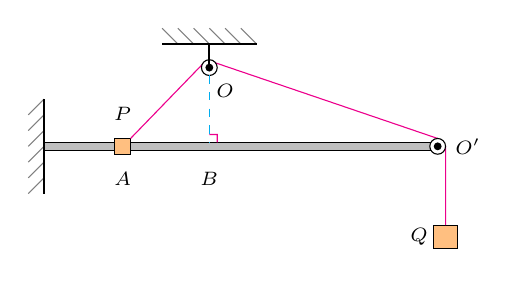
\begin{tikzpicture}[font=\scriptsize]
	\draw[fill=gray!50] (0,-.05) rectangle(5,.05);
	\draw[fill=orange!50] (.9,-.1) rectangle(1.1,.1) (4.95,-1) rectangle(5.25,-1.3);
	\draw[magenta] (1.1,.1)--(2.03,1.06) (2.12,1.08)--(5,.1) (5.1,0)--(5.1,-1) (2.2,.05)--(2.2,.15)--(2.1,.15);
	\draw[fill=white] (5,0) circle(.1) (2.1,1) circle(.1);
	\fill (2.1,1) circle(.05) (5,0) circle(.05);
	\foreach \y in {-.6,-.4,...,.6}
		\draw[gray] (-.2,\y)--++(.2,.2);
	\foreach \x in {1.5,1.7,...,2.5}
		\draw[gray] (\x,1.5)--++(.2,-.2);
	\draw[thick] (0,-.6)--(0,.6) (1.5,1.3)--(2.7,1.3) (2.1,1)--(2.1,1.3);
	\draw[dashed,cyan] (2.1,.9)--(2.1,.05);
	\node at(1,.2)[above]{\(P\)};
	\node at(1,-.2)[below]{\(A\)};
	\node at(2.1,-.2)[below]{\(B\)};
	\node at(5,-1.15)[left]{\(Q\)};
	\node at(5.1,0)[right]{\(O^{\prime}\)};
	\node at(2.3,.7){\(O\)};
\end{tikzpicture}
\begin{choices}
	\item 当物体\(P\)运动到\(B\)处时，此时物体\(P\)速度最小，物体\(Q\)速度最大
	\item 在物体\(P\)从\(A\)滑到\(B\)的过程中，物体\(P\)的机械能减小，物体\(Q\)的机械能增加
	\item 物体\(P\)运动的最大速度为\(\sqrt{6g(L - h)}\)
	\item 开始运动后，当物体\(P\)速度再次为零时，物体\(Q\)下降了\(2(L - h)\)
\end{choices}